% Results
\subsection{Aggregate Crime Variation}

The analysis of average provincial-level variations reveals a distinctive pattern in the response of criminal phenomena to pandemic-related restrictions. As shown in Table~\ref{tab:crime_variation_mean}, the offences considered can be clearly divided into two groups according to the type of interaction required for their commission. Contact-based crimes experienced sharp contractions, with pickpocketing recording the most pronounced decline ($-52.4\%$). This finding is consistent with the drastic reduction in urban mobility and tourist flows observed during the lockdown period. Residential burglaries ($-44.0\%$) and snatch thefts ($-38.6\%$) display similar trends, suggesting a strong correlation with reduced circulation in public spaces and increased time spent at home.By contrast, digital crimes registered substantial increases. Offences related to the possession of child sexual abuse material ($+86.3\%$) and cybercrime ($+83.2\%$) nearly doubled relative to the baseline period. Online fraud increased by $67.2\%$, reflecting the intensification of digital activity during the pandemic. The widespread adoption of smart working, distance learning, and e-commerce significantly expanded the pool of potential targets for cybercriminal communities.An apparently anomalous pattern emerges from the analysis of sexual violence ($+16.8\%$). Although classified as a contact-based crime, this offence exhibits a significant increase during the pandemic period. This countertrend is likely related to the situation of survivors\footnote{The term ``survivor'' is used here in an analytical sense to refer to individuals who have experienced sexual violence, in order to emphasise the continuity of subjectivity beyond the traumatic event and to avoid defining individuals exclusively through victimisation.}, who were often forced to cohabit with their abusers during lockdowns. It is important to stress that the positive variation in this indicator is particularly concerning, especially when considering the well-documented reporting bias associated with sexual and domestic violence. Sociological literature highlights how survivors of domestic violence were especially vulnerable during lockdowns, being confined at home with abusers\footnote{The term ``abuser'' is used to refer to the perpetrators of sexual violence in an analytical sense, with the aim of highlighting the relational and behavioural dimensions of violence, rather than reducing these individuals solely to the legal category of ``offender'' or ``criminal''.} and facing reduced access to support services \citep{koss1992}.

\begin{table}[htbp]
\centering
\caption{Percentage variation in average crime rates during the COVID period (2020--2021) compared to the pre-pandemic baseline (2014-2019). Values calculated across 107 Italian provinces.}
\label{tab:crime_variation_mean}
\begin{tabular}{lllc}
\toprule
\textbf{Istat code} & \textbf{Crime Type} & \textbf{Group} & \textbf{Mean variation (\%)} \\
\midrule
PICKTHEF & Pickpocketing & Contact & $-52.4$ \\
BURGTHEF & Residential burglary & Contact & $-44.0$ \\
BAGTHEF & Snatch theft & Contact & $-38.6$ \\
STREETROB & Street robbery & Contact & $-17.2$ \\
RAPE & Sexual assault & Contact & $+16.8$ \\
\midrule
PORNO & Child sexual abuse material & Digital & $+86.3$ \\
CYBERCRIM & Cybercrime & Digital & $+83.2$ \\
SWINCYB & Online fraud & Digital & $+67.2$ \\
\midrule
TOT & Total reported crimes & --- & $-16.8$ \\
\bottomrule
\end{tabular}
\end{table}

Overall, the total number of reported crimes decreased by $16.8\%$. This aggregate reduction, however, masks a substantial displacement effect: criminal activity largely shifted from physical spaces to the digital domain, supporting the hypothesis of mobility-restriction-induced crime displacement. Aggregation at the national level conceals marked territorial heterogeneity. The analysis of provincial distributions reveals that variations were far from uniform across the Italian territory. As shown in Table~\ref{tab:provincial_variations}, the provinces recording the highest relative increases include medium-sized and small areas located both in the North (Mantua, Ferrara, Lecco) and in the South (Avellino and Caltanissetta). This pattern suggests that the forced digitalisation induced by the pandemic affected territories with very different socio-economic characteristics. It can be hypothesised that these crimes impacted large Italian cities to a lesser extent, where digitalisation was already more advanced compared to provincial areas; however, given the available data, this remains a tentative interpretation.

% Cybercrime growth table
\begin{table}[htbp]
\centering
\caption{Provinces with the largest percentage increases in cybercrime rates during COVID (2020--2021).}
\label{tab:cybercrime_increases}
\begin{tabular}{lccc}
\toprule
\textbf{Provinces} & \textbf{Variation (\%)} & \textbf{Baseline (per 100k)} & \textbf{During COVID (per 100k)} \\
\midrule
Mantova & $+334.9$ & 33.6 & 146.3 \\
Avellino & $+301.8$ & 12.5 & 50.3 \\
Ferrara & $+244.9$ & 10.6 & 36.5 \\
Caltanissetta & $+213.5$ & 10.7 & 33.5 \\
Lecco & $+195.6$ & 13.7 & 40.6 \\
\bottomrule
\end{tabular}
\end{table}

The offence showing the largest relative increase concerns the possession of child sexual abuse material ($+86.3\%$ at the national level). While this figure warrants particular attention due to the intrinsic severity of the phenomenon, it must be interpreted with methodological caution. As shown in Table~\ref{tab:csam_increases}, baseline rates are extremely low (often below one offence per 100{,}000 inhabitants), making percentage variations highly sensitive to small absolute changes. Nevertheless, despite low absolute values, the generalised increase observed across the majority of Italian provinces points to a systematic phenomenon rather than statistical noise. This pattern is consistent with two non-mutually exclusive mechanisms: (i) increased online exposure of minors during lockdowns, and (ii) intensified production and distribution facilitated by prolonged domestic confinement and increased digital traffic.

% CSAM growth table
\begin{table}[htbp]
\centering
\caption{Provinces with the largest percentage increases in child sexual abuse material (CSAM) offence rates during COVID (2020--2021).}
\label{tab:csam_increases}
\begin{tabular}{lccc}
\toprule
\textbf{Province} & \textbf{Variation (\%)} & \textbf{Baseline (per 100k)} & \textbf{During COVID (per 100k)} \\
\midrule
Valle d'Aosta & $+700.0$ & 0.4 & 3.2 \\
Novara & $+485.7$ & 0.35 & 2.05 \\
Bari & $+451.6$ & 0.52 & 2.85 \\
Nuoro & $+368.8$ & 0.53 & 2.5 \\
Medio Campidano & $+368.8$ & 0.53 & 2.5 \\
\bottomrule
\end{tabular}
\end{table}

The most pronounced reductions in pickpocketing rates are observed in provinces characterised by strong commercial and touristic specialisation (Table~\ref{tab:pickpocketing_decreases}). Trieste ($-83.0\%$), Enna ($-82.0\%$), and Prato ($-72.7\%$) exhibit particularly large declines, in line with their role as commercial and tourist hubs. Milan, while also recording a substantial decrease ($-34.7\%$), displays a contraction well below the national average ($-52.4\%$). This suggests that, even under restrictive conditions, the Lombard metropolis maintained a residual level of urban activity and mobility higher than that observed in other territorial contexts.

% Pickpocketing degrowth table
\begin{table}[htbp]
\centering
\caption{Provinces with the largest percentage decreases in pickpocketing rates during COVID (2020--2021).}
\begin{tabular}{lccc}
\toprule
\textbf{Province} & \textbf{Variation (\%)} & \textbf{Baseline (per 100k)} & \textbf{During COVID (per 100k)} \\
\midrule
Trieste & $-83.0$ & 425.7 & 72.2 \\
Enna & $-82.0$ & 30.1 & 5.4 \\
Prato & $-72.7$ & 260.8 & 71.3 \\
Campobasso & $-69.1$ & 59.2 & 18.3 \\
Potenza & $-68.9$ & 35.1 & 10.9 \\
\bottomrule
\end{tabular}
\end{table}

\subsection{Spatial Autocorreletion Analysis}

The analysis of spatial autocorrelation using the global Moran’s I index reveals differentiated patterns in the spatial structure of criminal phenomena across the three periods considered. Table~\ref{tab:moran_values} reports Moran’s I values for the selected crime categories.

% Moran's values
\begin{table}[htbp]
\centering
\small
\caption{Global Moran's I and p-values for selected crime types, calculated at provincial level (NUTS-3) across temporal periods.}
\label{tab:moran_values}
\begin{adjustbox}{max width=\textwidth}
\begin{tabular}{lcccccc}
\toprule
\multirow{2}{*}{\textbf{Crime type}} & \multicolumn{2}{c}{\textbf{Pre-COVID (2014--2019)}} & \multicolumn{2}{c}{\textbf{During COVID (2020--2021)}} & \multicolumn{2}{c}{\textbf{Post-COVID (2022--2023)}} \\
\cmidrule(lr){2-3} \cmidrule(lr){4-5} \cmidrule(lr){6-7}
& Moran's I & p-value & Moran's I & p-value & Moran's I & p-value \\
\midrule
Pickpocketing & 0.198 & 0.003 & 0.191 & 0.009 & 0.092 & 0.060 \\
Residential burglary & 0.729 & 0.001 & 0.625 & 0.001 & 0.682 & 0.001 \\
Sexual assault & 0.338 & 0.001 & 0.373 & 0.001 & 0.446 & 0.001 \\
Cybercrime & 0.371 & 0.001 & 0.245 & 0.002 & 0.272 & 0.002 \\
Total crimes & 0.253 & 0.001 & 0.123 & 0.023 & 0.149 & 0.020 \\
\bottomrule
\end{tabular}
\end{adjustbox}
\end{table}

Pickpocketing exhibits a moderate degree of spatial clustering in the pre-pandemic period ($I = 0.198$, $p$-value $= 0.003$). This pattern remains relatively stable during the COVID period ($I = 0.191$, $p$-value $= 0.009$), but it almost completely dissolves in the post-COVID phase ($I = 0.092$, $p$-value $= 0.060$), losing statistical significance. Moran scatter plots (Figure~\ref{fig:moran_pickpocketing}) visually confirm this fragmentation. In the pre-COVID period, observations are concentrated along the regression line, with clearly identifiable High--High and Low--Low clusters. This structure persists during the lockdown period. In the post-pandemic phase, however, points display a marked dispersion around the regression line, indicating that pre-existing spatial patterns did not re-emerge. This is likely attributable to the slow recovery of the tourism sector, which plays a crucial role in pickpocketing activity.

\begin{figure}[htbp]
\centering
\includegraphics[width=0.95\textwidth]{figures/pickpocketing.png}
\caption{Moran scatter plots for pickpocketing across three periods.}
\label{fig:moran_pickpocketing}
\end{figure}

Cybercrime shows relatively high spatial clustering in the pre-pandemic period ($I = 0.371$, $p$-value $= 0.001$). This clustering weakens substantially during the pandemic ($I = 0.245$, $p$-value $= 0.002$) and then stabilizes in the post-COVID phase ($I = 0.272$, $p$-value $= 0.002$). Moran scatter plots (Figure~\ref{fig:moran_cybercrime}) reveal a crucial detail. In the pre-COVID period, several extreme High--High outliers appear in the upper-right quadrant, indicating provinces with very high cybercrime rates surrounded by similarly high-rate neighbors. During the COVID period, these extreme outliers move closer to the regression line, suggesting a more geographically homogeneous distribution. This pattern is consistent with the hypothesis that forced digitalization reduced territorial disparities in exposure to cybercrime, extending digital vulnerabilities to areas that were previously less affected.

\begin{figure}[htbp]
\centering
\includegraphics[width=0.95\textwidth]{figures/cybercrimes.png}
\caption{Moran scatter plots for cybercrime across three periods.}
\label{fig:moran_cybercrime}
\end{figure}

Sexual violence exhibits an anomalous and progressive increase in spatial clustering across all three periods ($I = 0.338 \rightarrow 0.373 \rightarrow 0.446$, all with $p$-values $< 0.01$). Unlike other contact-based crimes, which show attenuation or fragmentation of spatial patterns, sexual violence displays increasing geographic concentration. Moran scatter plots (Figure~\ref{fig:moran_sexual_violence}) show an increasingly tight alignment of observations along the regression line, with a strengthening of High--High clusters in the post-COVID period. This pattern suggests that pandemic-related factors may have amplified pre-existing territorial inequalities in either the reporting or incidence of sexual violence. As discussed in Section~4.1, this increase may reflect the inability of survivors to leave their homes while being forced into prolonged close contact with their abusers.

\begin{figure}[htbp]
\centering
\includegraphics[width=0.95\textwidth]{figures/rape.png}
\caption{Moran scatter plots for sexual assault across three preiods.}
\label{fig:moran_rape}
\end{figure}

Finally, Moran’s I computed on the total number of reported crimes shows a substantial reduction in overall spatial clustering during the COVID period (from $I = 0.253$ in the pre-COVID phase to $I = 0.123$ during COVID, both with $p$-values $< 0.05$). Moran scatter plots (Figure~\ref{fig:moran_total}) display a clear dispersion of observations away from the regression line during the pandemic, indicating that COVID-19 fragmented the overall spatial structure of crime. In the post-COVID period, a partial recovery is observed ($I = 0.149$), but clustering remains below pre-pandemic levels, suggesting that the spatial equilibria of crime have not fully returned to their previous configuration.

\begin{figure}[htbp]
\centering
\includegraphics[width=0.95\textwidth]{figures/total.png}
\caption{Moran scatter plots for total reported crimes across three periods.}
\label{fig:moran_total}
\end{figure}

\subsection{Local Spatial Cluster Dynamics}

While the global Moran’s I index quantifies overall spatial clustering, Local Indicators of Spatial Association (LISA) reveal where clusters are located and how they evolve geographically. LISA analysis classifies each province into four categories: High--High (HH) clusters, where high-crime provinces are surrounded by similarly high-rate neighbors; Low--Low (LL) clusters, where low-crime provinces aggregate; and spatial outliers (High--Low and Low--High). This section traces cluster transitions across the three periods, focusing on four representative crimes that exemplify distinct pandemic impacts.

Pickpocketing exhibits a dramatic spatial reconfiguration, with exceptionally low stability rates (Table~\ref{tab:lisa_pickpocketing}). The pre--post COVID stability of only 6.1\% indicates that the pandemic fundamentally altered the geography of this crime. In the pre-COVID period, hot spots were concentrated in the Ligurian coastal provinces (Genova, Savona, Imperia, La Spezia), along with scattered locations in Northern Italy. During COVID, six new hot spots emerged in the Po Valley region (Parma, Bologna, Ravenna, Firenze, Pistoia, Prato), while all Ligurian hot spots simultaneously disappeared—representing a complete cluster dissolution.

% LISA Pickpocketing Table
\begin{table}[htbp]
\centering
\caption{LISA cluster transitions for pickpocketing across pandemic periods.}
\label{tab:lisa_pickpocketing}
\begin{tabular}{lccc}
\toprule
\textbf{Metric} & \textbf{Pre $\to$ During} & \textbf{During $\to$ Post} & \textbf{Pre $\to$ Post} \\
\midrule
Hot Spots (total) & 11 & 10 & 10 \\
\quad New Hot Spots & +6 & +6 & +9 \\
Cold Spots (total) & 7 & 13 & 13 \\
\quad New Cold Spots & +2 & +9 & +7 \\
Disappeared Clusters & 3 & 6 & 6 \\
Stability Rate & 8.7\% & 7.0\% & 6.1\% \\
\bottomrule
\end{tabular}
\end{table}

The post-COVID period reveals no return to pre-pandemic patterns. Instead, nine new hot spots consolidated in Lombardy and Emilia-Romagna (Brescia, Bergamo, Verona, Cremona, Mantova, Ferrara, Bologna, Ravenna, Firenze), while Liguria remained non-significant. This permanent shift suggests that pickpocketing opportunities reorganized from coastal tourist centers to inland urban-industrial corridors. Such a transition likely reflects changes in mobility patterns, shifts in economic activity, or the slow recovery of international tourism, which historically characterized Ligurian hot spots. The expansion of cold spots was equally pronounced. Nine southern provinces transitioned into Low--Low clusters during COVID, signaling increasing spatial polarization between emerging northern clusters and a progressively low-crime South.

Cybercrime demonstrates moderate stability (20.9\% pre--post) accompanied by a clear geographic redistribution (Table~\ref{tab:lisa_cybercrime}). Pre-COVID hot spots were concentrated in Tuscany and Emilia-Romagna (Firenze, Pistoia, Prato, Modena, Bologna, Ferrara), forming a compact Central Italian cluster. During COVID, this cluster partially dissolved, with nine provinces losing hot-spot status, while five new hot spots emerged in the North-West (Varese, Novara, Cremona, Alessandria, Pavia).

% LISA Cybercrime table
\begin{table}[htbp]
\centering
\caption{LISA cluster transitions for cybercrime across pandemic periods.}
\label{tab:lisa_cybercrime}
\begin{tabular}{lccc}
\toprule
\textbf{Metric} & \textbf{Pre $\to$ During} & \textbf{During $\to$ Post} & \textbf{Pre $\to$ Post} \\
\midrule
Hot Spots (total) & 10 & 10 & 10 \\
\quad New Hot Spots & +5 & 0 & +4 \\
Cold Spots (total) & 23 & 13 & 13 \\
\quad New Cold Spots & +3 & +9 & +7 \\
Disappeared Clusters & 4 & 6 & 6 \\
Stability Rate & 21.7\% & 7.0\% & 20.9\% \\
\bottomrule
\end{tabular}
\end{table}

In the post-COVID period, this north-western cluster consolidated. Four provinces remained stable hot spots, whereas Tuscan and Emilian provinces definitively lost this status. Notably, no new hot spots emerged in the transition from during to post-COVID, suggesting that the phenomenon stabilized geographically after the initial pandemic reshuffling. This migration toward the North-West likely reflects differential rates of digitalization. Provinces characterized by advanced manufacturing and service sectors experienced more intense technological adoption during forced remote work, creating new vulnerability surfaces. The disappearance of Tuscan hot spots suggests that pre-COVID patterns may have reflected tourism-related cybercrime (e.g., credit card cloning or fraud targeting tourists), which collapsed during travel restrictions. By contrast, industrial digitalization in the North-West appears to have generated more persistent criminal opportunities.

Sexual violence exhibits the most concerning LISA pattern, with low initial stability (6.1\% pre--during) but progressive cluster consolidation rather than dissolution (Table~\ref{tab:lisa_rape}). Pre-COVID hot spots were limited and fragmented (Genova, Firenze, Prato, Trieste). During COVID, only one new hot spot emerged (La Spezia), while Genova and Firenze lost hot-spot status—an apparent weakening of clusters.

% LISA Sexual Assault Table
\begin{table}[htbp]
\centering
\caption{LISA cluster transitions for sexual assault across pandemic preiods.}
\label{tab:lisa_rape}
\begin{tabular}{lccc}
\toprule
\textbf{Metric} & \textbf{Pre $\to$ During} & \textbf{During $\to$ Post} & \textbf{Pre $\to$ Post} \\
\midrule
Hot Spots (total) & 5 & 13 & 12 \\
\quad New Hot Spots & +1 & +8 & +7 \\
Cold Spots (total) & 14 & 19 & 18 \\
\quad New Cold Spots & +11 & +5 & +12 \\
Disappeared Clusters & 3 & 2 & 2 \\
Stability Rate & 6.1\% & 16.5\% & 9.6\% \\
\bottomrule
\end{tabular}
\end{table}

However, the post-COVID period reveals a striking reversal. Eight new hot spots emerged (Cremona, Modena, Bologna, Lucca, Firenze, Pistoia, Prato, Pisa), forming a dense macro-cluster in Emilia-Romagna and Tuscany. Stability rates increased progressively (6.1\% $\rightarrow$ 9.6\% $\rightarrow$ 16.5\%), indicating a strengthening spatial structure. This sharply contrasts with other contact-based crimes such as pickpocketing, which experienced permanent cluster dissolution. This anomalous intensification aligns with two non-mutually exclusive hypotheses. First, under-reporting during lockdowns may have artificially deflated crime rates in provinces lacking robust support infrastructure, as survivors were confined with abusers and faced reduced access to services. Post-COVID reporting surges may then have concentrated in provinces with stronger institutional support, primarily in Central and Northern Italy. Second, pandemic-related stressors—economic hardship, social isolation, and prolonged domestic cohabitation—may have increased sexual violence in specific territorial contexts, with effects persisting beyond the pandemic.

Residential burglary displays the highest stability rates among all crimes analyzed (38.3\% pre--post), indicating that the pandemic minimally altered its spatial structure (Table~\ref{tab:lisa_residential_burglary}). A large and stable hot-spot cluster spanning Emilia-Romagna, Tuscany, Lombardy, and Veneto persisted across all three periods, with only marginal boundary adjustments.

% LISA Residential Burglary Table
\begin{table}[htbp]
\centering
\caption{LISA cluster transitions for residential burglary across pandemic preiods.}
\label{tab:lisa_residential_burglary}
\begin{longtable}{lccc}
\toprule
\textbf{Metric} & \textbf{Pre $\to$ During} & \textbf{During $\to$ Post} & \textbf{Pre $\to$ Post} \\
\midrule
Hot Spots (total) & 18 & 22 & 26 \\
\quad New Hot Spots & +2 & +7 & +7 \\
Cold Spots (total) & 28 & 29 & 29 \\
\quad New Cold Spots & +3 & +2 & +4 \\
Disappeared Clusters & 9 & 4 & 6 \\
Stability Rate & 35.7\% & 36.5\% & 38.3\% \\
\bottomrule
\end{longtable}
\end{table}

During COVID, this core temporarily contracted, as nine provinces lost hot-spot status (Torino, Cremona, Milano, Parma, Piacenza, Savona, Massa-Carrara, Imperia, Siena). However, post-COVID recovery was rapid and geographically proximate. Seven new hot spots emerged (Venezia, Verona, Padova, Lodi, Rovigo, Arezzo, Grosseto), most contiguous with the surviving central cluster. Notably, a metropolitan province such as Milano transitioned from HH (pre) to non-significant (during) and back to HH (post), demonstrating temporary pandemic suspension followed by the re-emergence of the structural pattern. The persistence of this Central-Northern macro-cluster, despite a 44\% reduction in intensity, reflects the dominance of structural factors over contingent disruptions. Residential burglary depends on territorial characteristics—housing typologies, urban density, highway accessibility enabling rapid escape routes, and proximity to regional borders—that lockdown measures did not fundamentally alter.

\begin{figure}
\centering
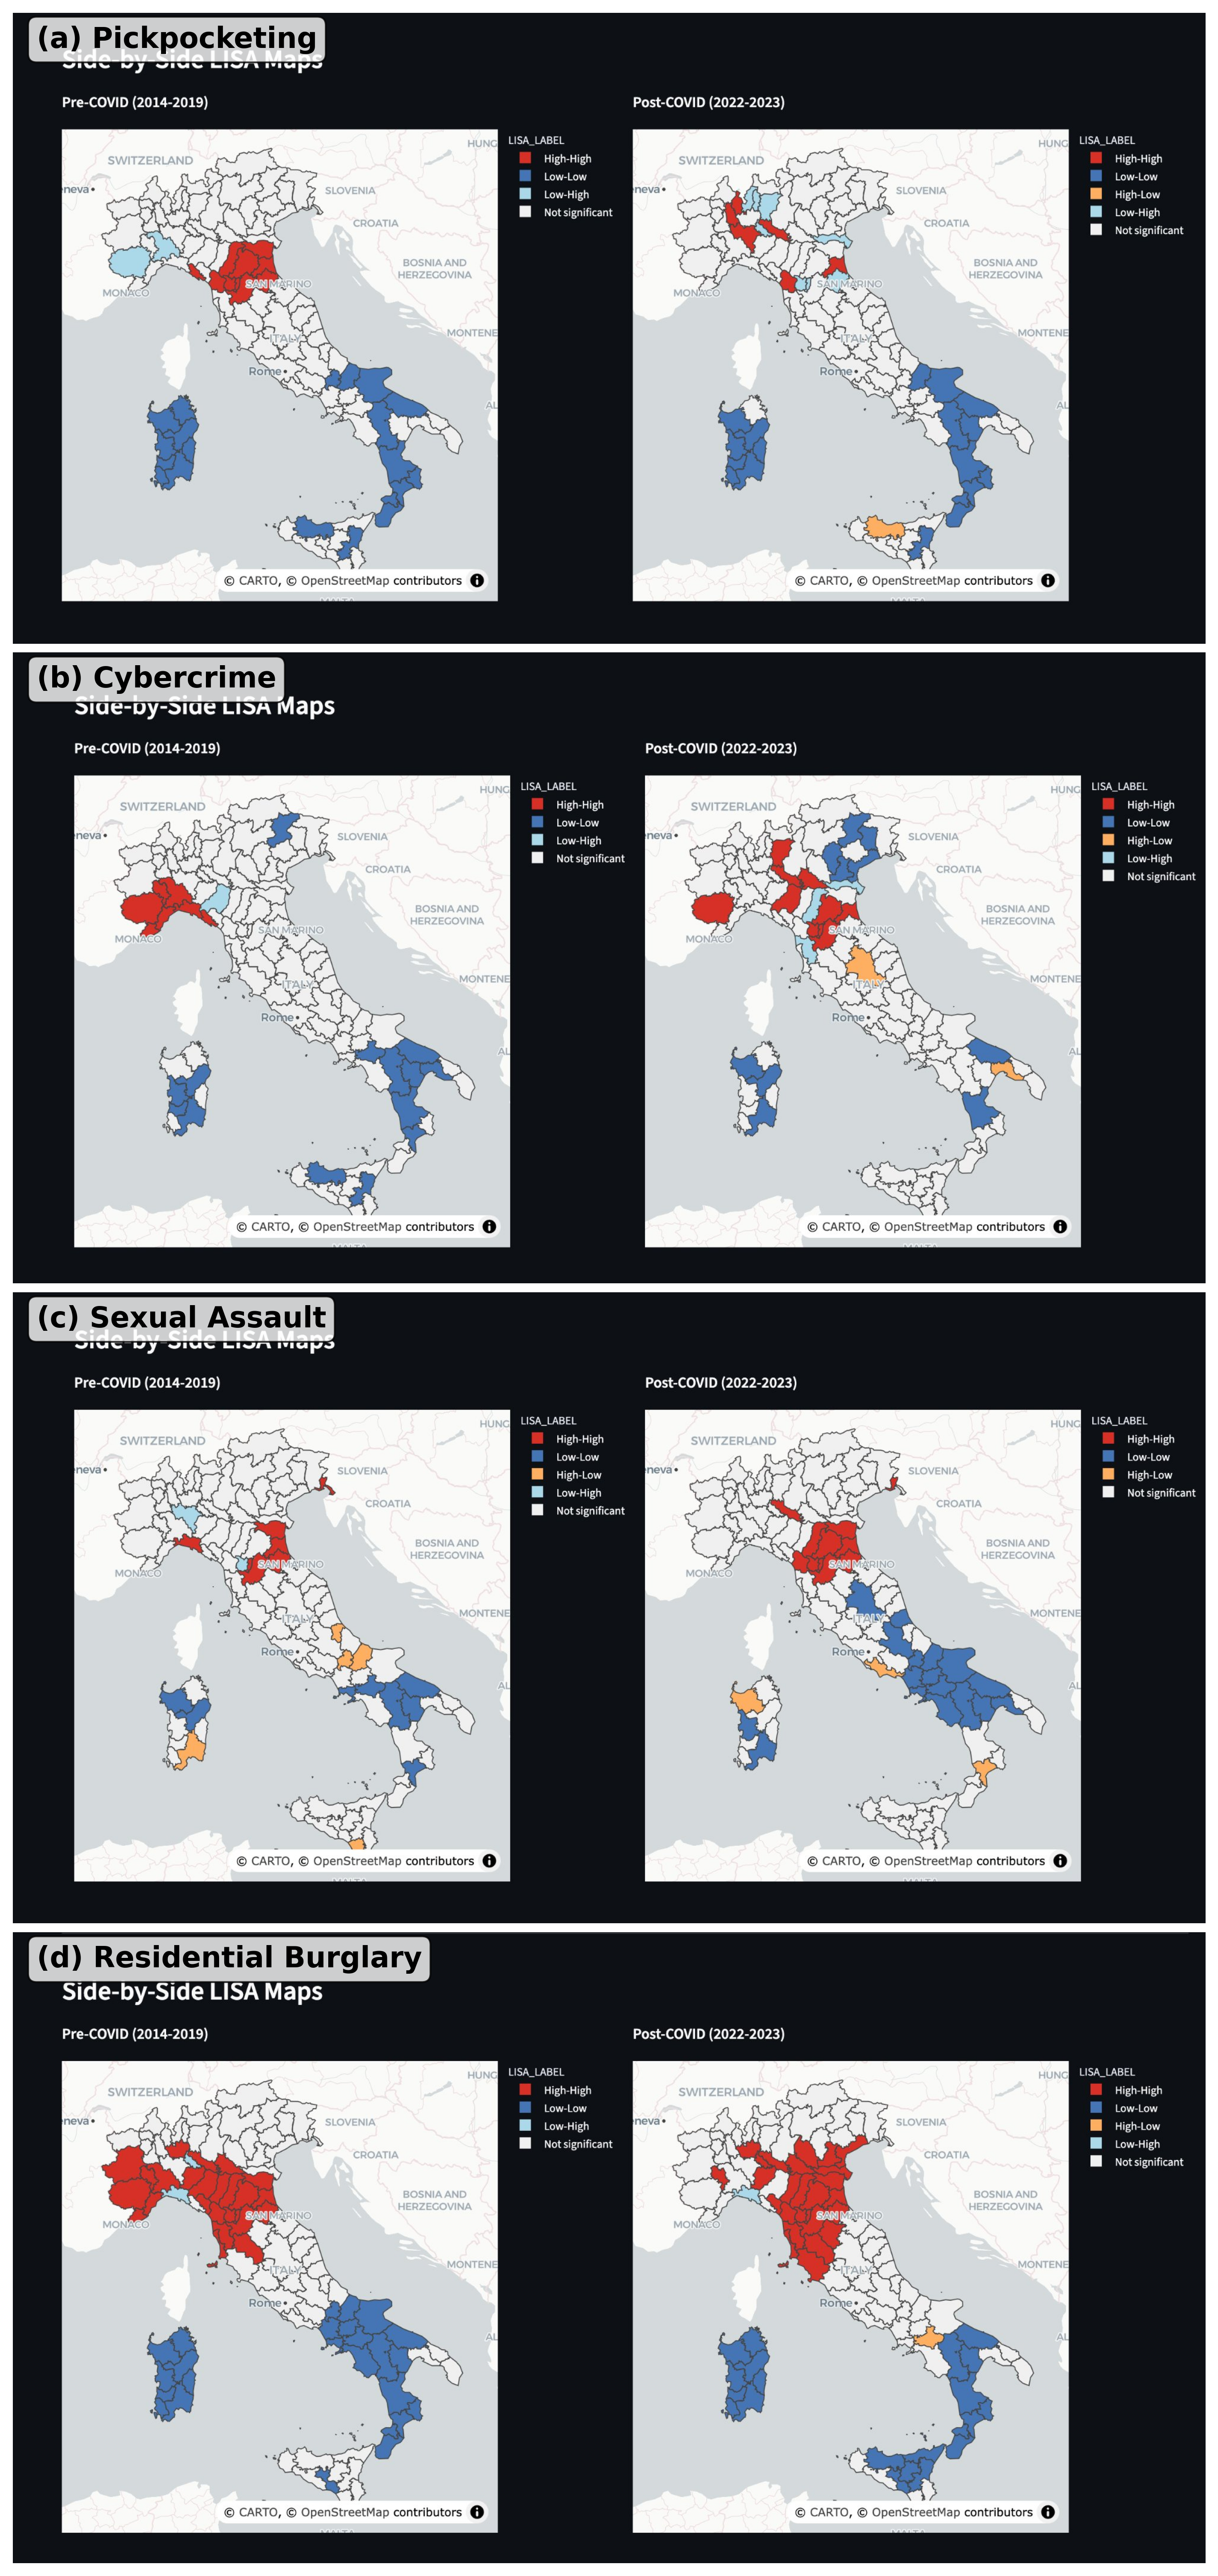
\includegraphics[
    width=\textwidth,
    height=0.9\textheight,
    keepaspectratio
]{figures/lisa_comparison.png}
\caption{LISA cluster configurations for four crime types comparing pre-COVID (2014--2019, left) and post-COVID (2022--2023, right) periods. (a) Pickpocketing; (b) Cybercrime; (c) Sexual assault; (d) Residential burglary.}
\label{fig:lisa_comparison}
\end{figure}

Figure~\ref{fig:lisa_comparison} visualizes these contrasting evolutionary trajectories across pre- and post-pandemic spatial configurations. The LISA analysis reveals three distinct patterns of cluster evolution. Opportunity-dependent crimes such as pickpocketing underwent permanent geographic reorganization, with stability rates below 10\% and no return to pre-pandemic configurations. Digital crimes such as cybercrime exhibited moderate stability (approximately 20\%), with clear spatial shifts reflecting uneven digitalization processes. Structural crimes such as residential burglary demonstrated high stability (above 35\%), with clusters contracting during restrictions but rapidly recovering in geographically proximate areas. Sexual violence stands apart. Its progressive clustering intensification differs from all other crime types and warrants dedicated investigation into reporting dynamics and territorial disparities in service provision. The contrast between the dissolution of pickpocketing and the persistence of residential burglary highlights a fundamental distinction: crimes dependent on mobile and transient populations (tourists, commuters) experienced lasting geographic disruption, whereas crimes rooted in residential and infrastructural patterns displayed remarkable resilience even under prolonged behavioral restrictions.
